\chapter{Example}\label{sec:example}

\section{Brain Sources Localization}\label{sec:BSL_example}
%\lstinputlisting{../../misc/demo/Brain_source_localization/BSL.m}



\paragraph{} An experience of Brain Source Localization using several gain matrices including FAuSTs and several solvers is provided. After configuring the matlab path (cf section \ref{sec:firstUseMatlabPath}). You can execute the matlab script \textbf{demo/Brain\_source\_localization/BSL.m} to run this experiment and \textbf{demo/Brain\_source\_localization/Fig\_BSL.m} to display the following pictures illustrating the speed-up using a Faµst.
In the Matlab terminal, you just need to type :
\begin{lstlisting}
>> BSL
>> Fig_BSL
\end{lstlisting}

Wich allows you to visualize this figure illustrating the speed-up with a Faust ($\mathbf{M}$ is the gain dense matrix and $\widehat{\mathbf{M}}_{6},\widehat{\mathbf{M}}_{9},\widehat{\mathbf{M}}_{16},\widehat{\mathbf{M}}_{26}$ are different Faust representing  $\mathbf{M}$):

\begin{figure}[!htbp]
\label{fig:BSL}
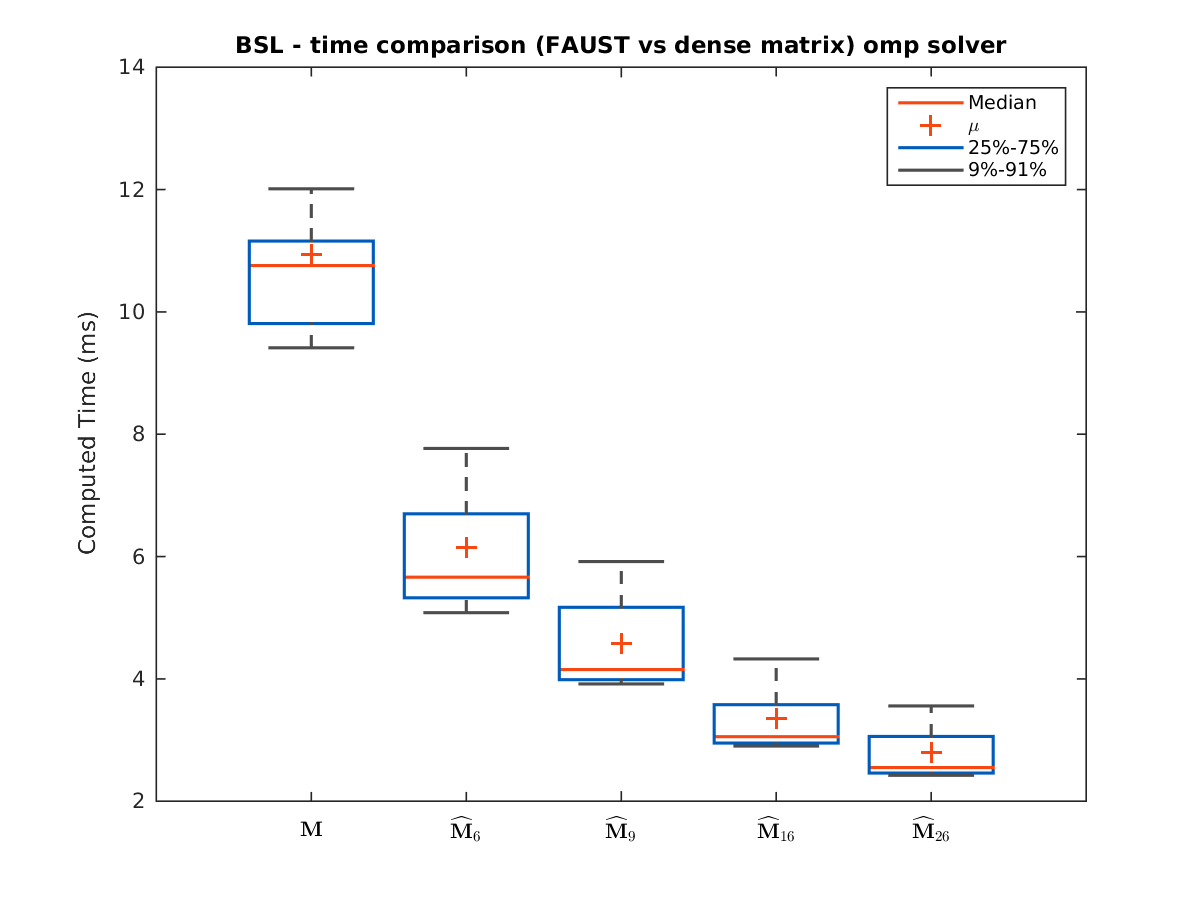
\includegraphics[scale=0.7]{images/BSL.png}
\end{figure}
